\documentclass[final]{transcrypto}
\usepackage[utf8]{inputenc}
\usepackage{amsmath}
\usepackage{amsfonts}
\usepackage{amssymb}
\usepackage{float}
\usepackage{caption}

\usepackage{physics}
\usepackage{amsmath}
\usepackage{tikz}
\usepackage{mathdots}
\usepackage{yhmath}
\usepackage{cancel}
\usepackage{color}
\usepackage{siunitx}
\usepackage{array}
\usepackage{multirow}
\usepackage{amssymb}
\usepackage{gensymb}
\usepackage{tabularx}
\usepackage{booktabs}
\usetikzlibrary{fadings}
\usetikzlibrary{patterns}

%% for code blocks
\usepackage{listings}
\usepackage{xcolor}



\begin{document}
%% Title
\title[short]{RECTANGLE Cipher}

%% Authors/affiliation:
\author{Abhiram \and Kausheek \and Manu}
\institute{Indian Institute of Technology, Bhilai\\ \email{ambatipudia@iitbhilai.ac.in } \and Indian Institute of Technology, Bhilai\\ \email{akellask@iitbhilai.ac.in} \and Indian Institute of Technology, Bhilai\\ \email{manue@iitbhilai.ac.in}}
\setDOI{}

%% Keywords/abstract:
\keywords{lightweight cryptography \and RECTANGLE \and bit-slice \and survey}
\begin{abstract}
In this paper, We present a survey and our study of block cipher named RECTANGLE. This cipher is a SPN block cipher with 16 $4\times 4$ Sbox for substituition and 3 rotations for permutation layer. A strong Sbox which has good hardware performance is chosen. The permutation layer of 3 rotations which is fast is used. RECTANGLE is made such that it can be efficiently implemented using bit slicing techniques. As a result it has good performance in both software and hardware. This paper covers overview, specifications, implementations, and attacks on this cipher. We also implemented both versions, bit slicing and normal-one in software (in Rust) and analyzed their performance. A lot of figures are added for easy visualization of the cipher's working and underlying operations.
\end{abstract}
\maketitle
\section{Introduction}
RECTANGLE was proposed as an improved lightweight symmetric cipher that performs well in both software and hardware. Prior to RECTANGLE there were many lightweight ciphers but none of them (except PRESENT which has some security weaknesses) had good performance in both software and hardware. Rectangle uses bit-slice techniques for fast execution; bit-slicing was used in improving software speed of DES and in implementation of Serpant cipher.

Because of rapidly increasing usage of embeded devices, IoT (Internet of Things) and other things, which require cipher for securing the data that is stored, transmitted and recieved, there is a huge demand for lightweight cipher. These devices generally have data that needs to be encrypted with moderately good cipher; using a good secure cipher like AES is not possible because of hardware limitations. These devices often run on low output low power or battery that has small capacity. Also these devices need to be small and fast so small circuits are used. At the time the time RECTANGLE was introduced there were no good lightweight ciphers that had good software performance. There were several good ciphers that had good hardware performance but their software performance is not good. Because of increased usage of lightweight ciphers there was a demand for new lightweight cipher that has good software performance.

TODO: after completion of paper, write about the structure of the paper.
\section{The Cipher}
Rectangle uses Substitution and Permutation Network (SPN) with  Each round consisting of S layer made of 16 $4 \times 4$ substitution boxes, P layer of 3 rotations and addition of round key (simple XOR of state matrix and round key).\\
\newline
Block length: 64 bits\\
Key length: 80 or 128 bits\\
\newline
\textbf{Encryption procedure:}\\
The input is 64 bit plaintext which is written as $4\times 16$ matrix. This matrix represents the "state". This matrix is iterated over several rounds and the initial state of this matrix is given plain text. And the final "state" matrix is the cipher text. Let the given plaintext be $v_{79}||v_{78}||v_{77}||\dots v_{0}$. Then state matrix will be:
$$S=
\begin{bmatrix}
v_{15} & v_{14} & v_{13} & \dots & v_{2} & v_{1} & v_{0}\\
v_{31} & v_{30} & v_{29} & \dots & v_{18} & v_{17} & v_{16}\\
v_{47} & v_{46} & v_{45} & \dots & v_{34} & v_{33} & v_{32}\\
v_{63} & v_{62} & v_{61} & \dots & v_{50} & v_{49} & v_{48}\\
\end{bmatrix}
$$
We also use the following notation for state matrix:
$$
\begin{bmatrix}
a_{0,15} & a_{0,14} & a_{0,13} & \dots & a_{0,2} & a_{0,1} & a_{0,0}\\
a_{1,15} & a_{1,14} & a_{1,13} & \dots & a_{1,2} & a_{1,1} & a_{1,0}\\
a_{2,15} & a_{2,14} & a_{2,13} & \dots & a_{2,2} & a_{2,1} & a_{2,0}\\
a_{3,15} & a_{3,14} & a_{3,13} & \dots & a_{3,2} & a_{3,1} & a_{3,0}\\
\end{bmatrix}
$$
Where $row_{i} = a_{15,i}||a_{14,i}||a_{13,i}||..a_{0,0}$\\
The algorithm for encryption is as follows:
\begin{lstlisting}[float,floatplacement=H]
state = PlainText;
subkey = IV_key;
for i in 0..26 {
    AddRoundKey(state, subkey);
    SubColumn(state);
    ShiftRow(state);
    subkey = NextSubKey(subkey, i);
}
AddRoundKey(state, subkey);
CipherText = state; 
\end{lstlisting}\\
\newline
There are 25 rounds and a final XOR. Following functions are used in each round:\\
AddRoundKey: State matrix is XORed with round subkey.\\
SubColumn: Each column of state is passed Sbox (Substitution layer)\\
ShiftRow: Each row of the state is rotated (Permutation layer)\\
NextSubKey: Next round's subkey is obtained using key schedule, see \ref{KeySchedule} for more details.\\
Detailed working of algorithm is decsribed in \ref{Rounds}.
\subsection{Key Schedule}
\label{KeySchedule}
\subsubsection{80 bit key version:}
Make a key state matrix that is $5\times 16$ matrix from the given initial key (KeyIV).\\
Let the given key be $IV = v_{79}||v_{78}||v_{77}||\dots v_{0}$. Then the initial key state matrix will be as follows:
$$
\begin{bmatrix}
v_{15} & v_{14} & v_{13} & \dots & v_{2} & v_{1} & v_{0}\\
v_{31} & v_{30} & v_{29} & \dots & v_{18} & v_{17} & v_{16}\\
v_{47} & v_{46} & v_{45} & \dots & v_{34} & v_{33} & v_{32}\\
v_{63} & v_{62} & v_{61} & \dots & v_{50} & v_{49} & v_{48}\\
v_{79} & v_{78} & v_{77} & \dots & v_{66} & v_{65} & v_{64}\\
\end{bmatrix}
$$
Let us the following notation for elements of the key matrix:
$$
\begin{bmatrix}
k_{0,15} & k_{0,14} & k_{0,13} & \dots & k_{0,2} & k_{0,1} & k_{0,0}\\
k_{1,15} & k_{1,14} & k_{1,13} & \dots & k_{1,2} & k_{1,1} & k_{1,0}\\
k_{2,15} & k_{2,14} & k_{2,13} & \dots & k_{2,2} & k_{2,1} & k_{2,0}\\
k_{3,15} & k_{3,14} & k_{3,13} & \dots & k_{3,2} & k_{3,1} & k_{3,0}\\
k_{4,15} & k_{4,14} & k_{4,13} & \dots & k_{4,2} & k_{4,1} & k_{4,0}\\
\end{bmatrix}
$$
$i^{th}$ row is $row_{i} = k_{15,i}||k_{14,i}||k_{13,i}||..k_{0,0}$\\
\newline
The following operations are applies $i$ times to obtain subkey of $i^{th}$ round:\\
\textbf{NextSubKey():}\\
\begin{enumerate}
    \item S-box is applied to 4 rightmost columns (4 rows) i.e.,
$$k'_{3,i}||k'_{2,i}||k'_{1,i}||k'_{1,i} = Sbox[k_{3,i}||k_{2,i}||k_{1,i}||k_{1,i}]$$ for $i=\{0,1,2,3\}$.
    \item Feistal transformation is applied as follows:
$row'_0 = (row_0\ll 8)\oplus row_1$\\
$row'_1 = row_2$\\
$row'_2 = (row_2\ll 16)\oplus row_3$\\
$row'_3 = row_0$\\
    \item Last five bits of keystate are XORed with round constant of current round.\\
\end{enumerate}

The below figure represents sbox operation. In this figure each block represents 4 bits. After the sbox operation it can be seen that top 4 rows of right most column are darkened because they are modified by the sbox.
\begin{figure}[H]
\caption{Sbox}
\centering
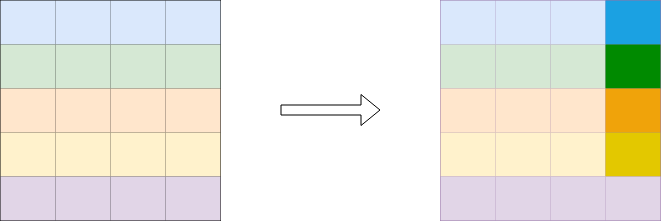
\includegraphics[width=0.85\textwidth]{images/key_s_sbox.png}
\end{figure}
The below figure shows Feistal transformation. Matrix on the top right is the original matrix with rows circularly rotated by one(downward). Matrix on the left bottom is the orginal matrix with all rows deleted except 0th and 3rd, which are left shifted by 8 and 12 respectively. (note here each block represents 4 bits)
\begin{figure}[H]
\caption{Sbox}
\centering
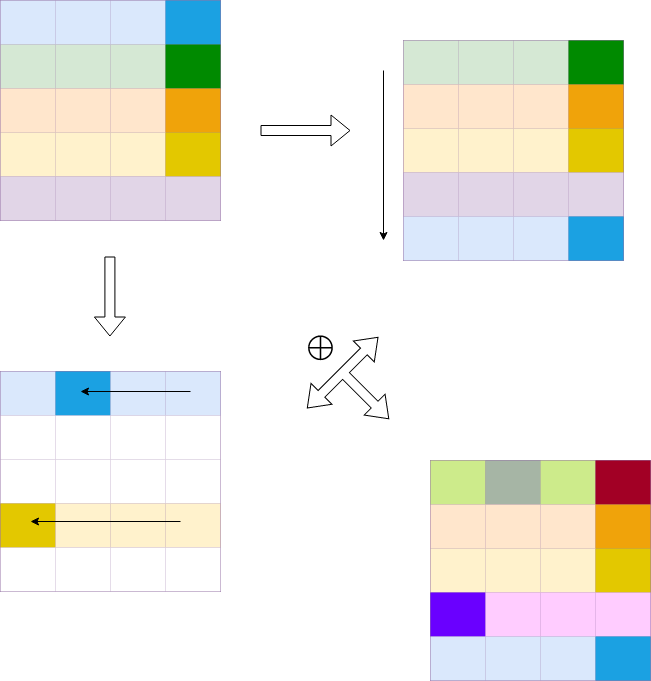
\includegraphics[width=0.85\textwidth]{images/key_s_f.png}
\end{figure}
Finally, round constants are applied to rightmost 5 bits of first row.
\begin{figure}[H]
\caption{Sbox}
\centering
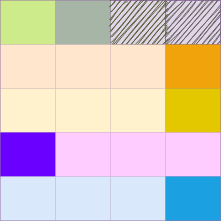
\includegraphics[width=0.26\textwidth]{images/key_s_rc.png}
\end{figure}
\subsubsection{For 128 bit verison:}
Procedure for 128 bit is similar to 80 bit with small differences, here key state matrix is $4\times 32$ matrix instead of $5\times 16$.\\
1. S-box is applied to 8 rightmost columns.\\
2. Fiestal transformation is applied as follows:\\
$row_0 = (row_0\ll 8)\oplus row_1$\\
$row_1 = row_2$\\
$row_2 = (row_2\ll 16)\oplus row_3$\\
$row_3 = row_0$\\
3. XOR is same i.e., last five bits of keystate are XORed with round constant of current round.
\subsection{S-box}
\begin{table}[H]
	\centering
	\caption{S-box}
	\begin{tabular}{|l|l|l|l|l|l|l|l|l|l|l|l|l|l|l|l|l|}
		\hline
 $x$&0&1&2&3&4&5&6&7&8&9&a&b&c&d&e&f\\ \hline
$S(x)$&6&5&c&a&1&e&7&9&b&0&3&d&8&f&4&2 \\ \hline

	\end{tabular}
\end{table}
\subsection{Rounds}
\label{Rounds}
Following operations are applied in each round.\\
\textbf{AddRoundKey}\\
State matrix is XORed with roundkey.\\
(Note: In the following figures used for Rounds section, each block represents one bit)
\begin{figure}[H]
\caption{AddRoundKey}
\centering
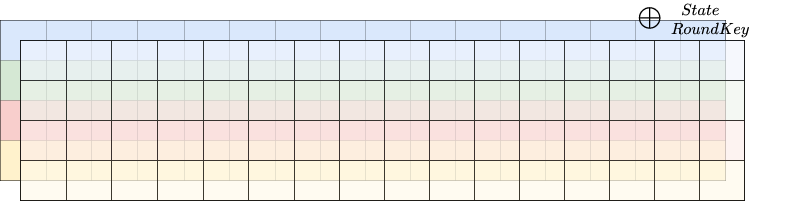
\includegraphics[width=0.85\textwidth]{images/round_xor.png}
\end{figure}
Each column of state is passed through Sbox. This operation (SubColumn) can be efficiently implemented using bitslicing instead of using Sbox on each column.
\textbf{SubColumn}\\
\begin{figure}[H]
\caption{SubColumn}
\centering
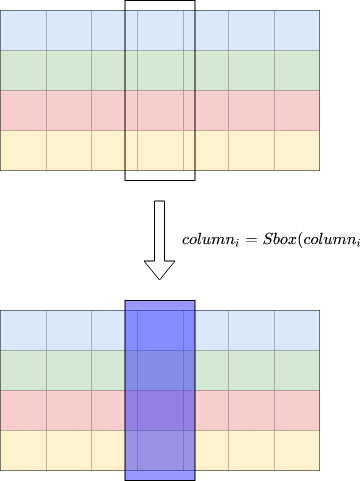
\includegraphics[width=0.45\textwidth]{images/round_sbox.png}
\end{figure}
0th row is unmodified. 1st row is left (circular) shifted by 1. 2nd row is left (circular) shifted by 12. And 3rd row is left (circular) shifted by 13.\\
\textbf{ShiftRow}\\
\begin{figure}[H]
\caption{ShiftRow}
\centering
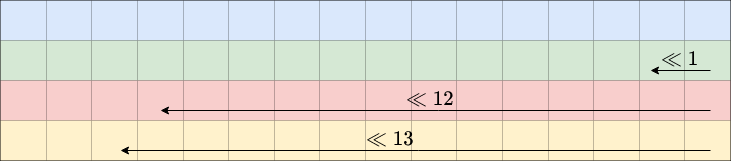
\includegraphics[width=0.85\textwidth]{images/round_shift.png}
\end{figure}

\section{Implementation}
Both bitslicing and normal versions of RECTANGLE cipher are implemented in Rust (no dependencies).
see "implementations" directory for implemnetaion files.
\section{Cryptanalysis}
\subsection{S-box}
A good (no security weakness) S-box is choosen that has good hardware performance (low area).
\subsection{DDT}
We can see that the Sbox is good as there are no combinations of input-output difference for which there more than 4 pairs.
see "cryptanalysis" directory for code of DDT (Implemented in python3).
\begin{table}[H]
	\centering
	\caption{DDT of S-box}
	\begin{tabular}{|l||l|l|l|l|l|l|l|l|l|l|l|l|l|l|l|l|}
		\hline
 &  0&	1&	2&	3&	4&	5&	6&	7&	8&	9&	a&	b&	c&	d&	e&	f\\ \hline
 \hline
0& 16 & 0 & 0 & 0 & 0 & 0 & 0 & 0 & 0 & 0 & 0 & 0 & 0 & 0 & 0 & 0 \\ \hline
1& 0 & 0 & 0 & 2 & 0 & 0 & 4 & 2 & 0 & 0 & 0 & 2 & 0 & 0 & 4 & 2 \\ \hline
2& 0 & 0 & 0 & 0 & 0 & 0 & 2 & 2 & 2 & 0 & 2 & 0 & 2 & 4 & 0 & 2 \\ \hline
3& 0 & 0 & 0 & 2 & 0 & 0 & 2 & 0 & 2 & 4 & 2 & 2 & 2 & 0 & 0 & 0  \\ \hline 
4& 0 & 0 & 0 & 4 & 0 & 0 & 0 & 4 & 0 & 0 & 0 & 4 & 0 & 0 & 0 & 4  \\ \hline
5& 0 & 2 & 0 & 0 & 4 & 2 & 0 & 0 & 4 & 2 & 0 & 0 & 0 & 2 & 0 & 0  \\ \hline
6& 0 & 2 & 4 & 0 & 2 & 0 & 0 & 0 & 0 & 0 & 0 & 2 & 2 & 2 & 0 & 2  \\ \hline
7& 0 & 0 & 4 & 0 & 2 & 2 & 0 & 0 & 0 & 2 & 0 & 2 & 2 & 0 & 0 & 2  \\ \hline
8& 0 & 2 & 0 & 2 & 0 & 2 & 0 & 2 & 0 & 2 & 0 & 2 & 0 & 2 & 0 & 2  \\ \hline
9& 0 & 2 & 0 & 0 & 0 & 2 & 4 & 0 & 0 & 2 & 0 & 0 & 0 & 2 & 4 & 0  \\ \hline
a& 0 & 0 & 0 & 0 & 0 & 4 & 2 & 2 & 2 & 0 & 2 & 0 & 2 & 0 & 0 & 2  \\ \hline
b& 0 & 4 & 0 & 2 & 0 & 0 & 2 & 0 & 2 & 0 & 2 & 2 & 2 & 0 & 0 & 0  \\ \hline
c& 0 & 0 & 0 & 0 & 4 & 0 & 0 & 0 & 4 & 0 & 4 & 0 & 0 & 0 & 4 & 0  \\ \hline
d& 0 & 2 & 0 & 0 & 0 & 2 & 0 & 0 & 0 & 2 & 4 & 0 & 0 & 2 & 4 & 0  \\ \hline
e& 0 & 0 & 4 & 2 & 2 & 2 & 0 & 2 & 0 & 2 & 0 & 0 & 2 & 0 & 0 & 0  \\ \hline
f& 0 & 2 & 4 & 2 & 2 & 0 & 0 & 2 & 0 & 0 & 0 & 0 & 2 & 2 & 0 & 0 \\ \hline
	\end{tabular}
\end{table}

\subsection{LAT}
We can see that the Sbox is good as there are no bias values exceeding 4.
see "cryptanalysis" directory for code of LAT (Implemented in ruby).
\begin{table}[H]
	\centering
	\caption{LAT of S-box}
	\begin{tabular}{|l||l|l|l|l|l|l|l|l|l|l|l|l|l|l|l|l|}
		\hline
&0&1&2&3&4&5&6&7&8&9&a&b&c&d&e&f\\ \hline
\hline
0&+8&.&.&.&.&.&.&.&.&.&.&.&.&.&.&.\\ \hline
1&.&.&.&+4&.&-4&.&.&+2&-2&-2&-2&-2&-2&+2&-2\\ \hline
2&.&.&.&.&.&.&+4&+4&.&.&+4&-4&.&.&.&.\\ \hline
3&.&.&.&-4&+4&.&.&.&-2&+2&-2&-2&-2&-2&+2&-2\\ \hline
4&.&.&.&.&.&.&-4&+4&.&.&.&.&.&.&+4&+4\\ \hline
5&.&.&-4&.&.&-4&.&.&-2&+2&-2&-2&+2&+2&-2&+2\\ \hline
6&.&.&.&.&.&.&.&.&+4&+4&.&.&-4&+4&.&.\\ \hline
7&.&.&-4&.&-4&.&.&.&-2&+2&+2&+2&-2&-2&+2&-2\\ \hline
8&.&.&.&-4&-2&-2&+2&-2&.&-4&.&.&-2&+2&+2&+2\\ \hline
9&.&.&.&.&-2&+2&+2&-2&+2&+2&-2&-2&+4&.&+4&.\\ \hline
a&.&.&.&-4&-2&-2&-2&+2&+4&.&.&.&+2&-2&-2&-2\\ \hline
b&.&.&.&.&+2&-2&+2&-2&+2&+2&+2&+2&.&-4&.&+4\\ \hline
c&.&+4&.&.&-2&+2&-2&-2&.&.&.&-4&-2&-2&-2&+2\\ \hline
d&.&+4&+4&.&-2&-2&+2&+2&-2&+2&-2&+2&.&.&.&.\\ \hline
e&.&-4&.&.&-2&+2&+2&+2&.&.&-4&.&-2&-2&-2&+2\\ \hline
f&.&+4&-4&.&+2&+2&+2&+2&+2&-2&-2&+2&.&.&.&.\\ \hline
	\end{tabular}
\end{table}
\subsection{Linear Cryptanalysis}
RECTANGLE is resistant to linear cryptanalysis attacks. Maximum number of rounds that can be attacked using linear cryptanalysis is 14. Also there no clustering of linear trails which can make effective distinguisher for 15 rounds.\\
These estimation are obtained as follows. If $\epsilon$ is the bias for a liner trail then the correlation contribution is $2\epsilon$.
\textbf{Theorem 1}. The square of a correlation (or correlation contribution) is called correlation potential.The average correlation potential between an input and an output selection pattern is the sum of the correlation potentials of all linear trails between the input and output selection patterns:
$$E(C_t^2) = \sum (C_i)^2$$ 

where $C_t$ is the overall correlation, and $C_i$ is the correlation coefficitent of linear trail.
\subsection{Differential Cryptanalysis}
RECTANGLE is resistant to differential cryptanalysis attacks. Maximum number of rounds that can be attacked using differential cryptanalysis is 18, 18 round distinguisher(using 14 round differnect propogation).\\
Since we are using a 64 bit key we need a difference propogation with probability of atleast $2^{-63}$.
The authors of RECTANGLE's paper used a modified version of M. Matsui's search algorithm for finding all differential/linear trials which uses branch and bound method. Best differential trails from round 1 to round 15 are obtaind using this algorithm. Results of the search are as follows:
\begin{enumerate}
 \item here are 32 best difference propagations with probability $1300\times 2^{-76}\approx 2^{-65.66}$ each. Each is composed of 7 differential trails. Among the 7 trails, one with probability $2^{66}$, two with probability $2^{69}$each,one with probability $2^{72}$, one with probability $2^{75}$, and two with probability $2^{76}$ each.
    \item Among all the difference propagations, the maximum number of trails of a difference propagation is 131,i.e., a difference propagation is composed of at most 131 different differential trails. For such a difference propagation, the probability is $421\times 2^{76}\approx 2^{67.28}$

\end{enumerate}
We can see that there are no differnece propogations that have probabitlity higher than $2^{-63}$ and there is low clustering of trails. Therefore we can not construct a difference propogation for more than 14 rounds.
\subsection{Differnece Propogation}
\begin{figure}[H]
\caption{Example Difference propogation 1}
\centering
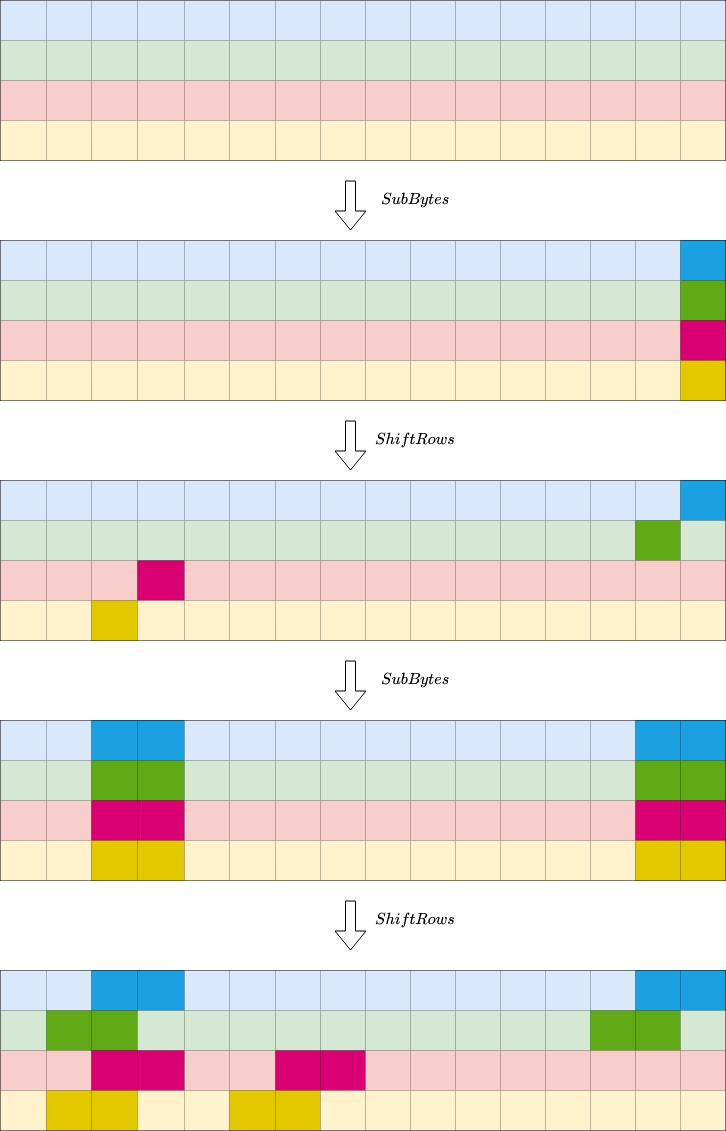
\includegraphics[width=0.85\textwidth]{images/diff_prop1_xor.png}
\end{figure}
\begin{figure}[H]
\caption{Example Difference propogation 2}
\centering
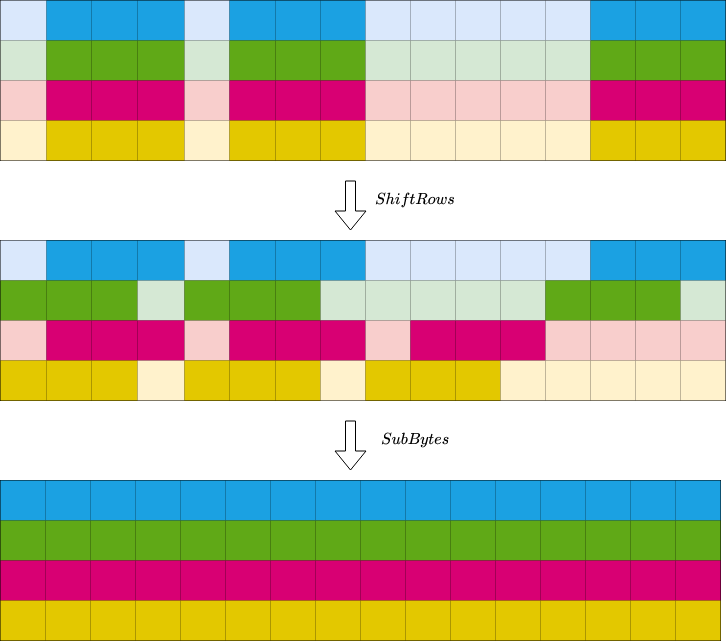
\includegraphics[width=0.85\textwidth]{images/diff_prop2_xor.png}
\end{figure}


\section{Performance}
Both the software and hardware performaces of RECTANGLE are impressive. 
\subsection{Hardware Implementation Performance}

\subsection{Software Implementation Performance}

\section{Conclusion}


\section{Brownie Point Nomination}
1. A lot of images are used to help visualize the operations applied.\\
2. Performance comparision of bit-slicing vs normal version is done in software implementation.\\
3. Encryption Algorithm is explained in much more detailed way and is easy to understand.\\


TODO:\\
add new changes from: \href{https://www.cryptolux.org/index.php/Lightweight_Block_Ciphers#Rectangle}{rect}\\
add reference: \href{https://www.researchgate.net/figure/S-box-design-consideration_tbl4_280218646}{rg}\\
ref of above one: Bansod, Dr. Gaurav. (2015). PICO: An Ultra lightweight and Low power encryption design for pervasive computing. eprint.iacr.org. 10.1631/FITEE.1500415. \\

2. osuge H, Tanaka H, Iwai K, et al.  Integral attack on reduced-round Rectangle.  In: Proceedings of IEEE 2ndInternational Conference on Cyber Security and Cloud Computing (CSCloud), 2015. 68–73\\


\begin{thebibliography}{9}
\bibitem{rectangle}
Wentao Zhang, Zhenzhen Bao, DongdaiLin, Vincent Rijmen, Bohan Yang, Ingrid Verbauwhede. RECTANGLE: A Bit-slice Lightweight Block CipherSuitable for Multiple Platforms. SCIENCE CHINA Information Sciences, December, 2015, Vol. 58: 122103(15), \href{https://www.doi.org/10.1007/s11432-015-5459-7}{doi: 10.1007/s11432-015-5459-7}

\bibitem{relatedKey}
Jinyong Shan, Lei Hu, Ling Song, Siwei Sun, and Xiaoshuang Ma. Related-Key Differential Attack on RoundReduced RECTANGLE-80.  Journal of Cryptologic Research, 2015, 2(1): 54-65. \href{http://www.jcr.cacrnet.org.cn/EN/Y2015/V2/I1/54}{http://www.jcr.cacrnet.org.cn/EN/Y2015/V2/I1/54}

\bibitem{imprAttack}
Asuman Senol. Improved Differential Attacks on RECTANGLE. The Graduate School of Informatics of Middle East Technical University. August 2017. \href{http://www.cihangir.forgottenlance.com/files/asuman_senol_master_thesis.pdf}{http://www.cihangir.forgottenlance.com/files/asuman\_senol\_master\_thesis.pdf}
\end{thebibliography}
\end{document}
